% Motivation for the study of Gravitational Waves

This thesis focuses on research made to improve our capability to detect gravitational waves. While the research targeted data quality and gravitational wave searches, it is useful to introduce gravitational waves in this chapter. In this chapter a broad overview of general relativity, compact binary coalescence signals and interferometers is given and is not intended to describe fully the workings and background of these topics. The derivation of gravitational waves closely follows the textbook `A General Relativity Workbook' by Thomas A. Moore \cite{moore_2013}.

In this chapter we begin by introducing the concept of gravitational waves and their derivation from general relativity in section~\ref{1:sec:gravitational-radiation}. In section~\ref{} we discuss the primary source of gravitational wave that is observable in the modern gravitational wave detector era, compact binary coalescence. In section~\ref{} we discuss the construction of gravitational wave interferometers and how they are able to observe gravitational waves. Finally, in section~\ref{} we discuss the effects of gravitational wave astronomy on the wider astronomy field and how gravitational wave observations can be harnessed in tandem with other sources to provide greater information about astrophysical events.

\section{\label{1:sec:gravitational-radiation}Gravitational radiation}

% Introduce the Section
In this section we will briefly introduce gravitational radiation.

\subsection{\label{1:sec:perturbations}Perturbations in spacetime}
%     Concept of Gravitational Waves: Describe what gravitational waves are and how they arise as perturbations in spacetime.

% Introduce Einstein Field Equations
The Einstein field equations (Einstein's equations) are a set of $10$ equations which, for a point in spacetime, relate the curvature of spacetime and the density of matter and energy. General relativity introduces the standard tensor notation, in which we can write Einstein's equations as
%
\begin{equation}
   R_{\mu \nu} - \frac{1}{2}g_{\mu \nu}R = 8 \pi G T_{\mu \nu}
   \label{2:eqn:EFE}
\end{equation}
%
where $R_{\mu \nu}$ is the Ricci tensor, $R$ the Ricci scalar and $g_{\mu \nu}$ the 4-dimensional spacetime metric tensor. $T^{\mu \nu}$ is the stress energy tensor which describes the density and flux of matter, energy and momentum. We note that $R_{\mu \nu}$, $g_{\mu \nu}$ and $T_{\mu \nu}$ are all symmetric and therefore Einstein's equations consist of only $10$ equations rather than $16$.

% Small Perturbations in Spacetime
We consider the case where a \textit{weak} gravitational field exists in a flat spacetime to simplify Einstein's equations. In this case the spacetime metric tensor, $g_{\mu\nu}$, can be expressed as the sum of a small perturbation due to the gravitational field, $h_{\mu\nu}$, and the flat space Minkowski metric tensor $\eta_{\mu\nu}$,
%
\begin{equation}
g_{\mu\nu} = \eta_{\mu\nu} + h_{\mu\nu}, \quad |h_{\mu\nu}| \ll 1.
\end{equation}
%
We have ensured that our gravitational field is weak by considering only perturbations with magnitude far smaller than unity.

% Linearized Gravity
With such a small perturbation the Einstein field equations can then be linearised by ignoring non-linear terms in $h_{\mu\nu}$, due to their negligible magnitude, this is known as taking the weak field limit. We are then able to simplify the left-hand side of equation~\ref{2:eqn:EFE} in the weak field limit,
%
\begin{equation}
    R_{\mu\nu} - \frac{1}{2}g_{\mu\nu}R = \frac{1}{2}\left(\partial^{\sigma}\partial_{\mu}\Bar{h}_{\sigma\nu} - \partial^{\sigma}\partial_{\sigma}\Bar{h}_{\mu\nu} + \partial_{\nu}\partial^{\alpha}\Bar{h}_{\mu\alpha} - \eta_{\mu\nu}\partial^{\alpha}\partial^{\beta}\Bar{h}_{\alpha\beta}\right) ,
\end{equation}
%
where $\Bar{h}_{\mu\nu}$ is defined as the ``trace reverse'' of $h_{\mu\nu}$,
%
\begin{equation}
    \Bar{h}_{\mu\nu} = h_{\mu\nu} - \frac{1}{2}\eta_{\mu\nu}h_{\alpha}^{\alpha} ,
    \label{2:eq:trace-reverse-h}
\end{equation}
%
and the indices of $h_{\mu\nu}$ can be raised or lowered by multiplication with just $\eta_{\mu\nu}$,
%
\begin{equation}
    h^{\alpha\beta} = \eta^{\alpha\mu}\eta^{\beta\nu}h_{\mu\nu} .
\end{equation}
%

\subsection{\label{1:sec:weak-field}Weak field approximations}
%    Weak Field Approximation

% Gauge Transformations
To further simplify our derivation of gravitational waves we can consider the gauge transformation in the weak field and apply small coordinate translations to the perturbed spacetime. These coordinate translations keep the metric perturbations small,
%
\begin{equation}
    x^{\prime\mu} = x^{\mu} + \xi^{\mu}(x) .
\end{equation}
%
We can then define the metric in the new coordinate system which will transform according to,
%
\begin{equation}
    g^{\prime}_{\mu\nu}(x^{\prime}) = \frac{\delta x^{\rho}}{\delta x^{\prime\mu}} \frac{\delta x^{\sigma}}{\delta x^{\prime\nu}}  g_{\rho\sigma}(x) = \eta_{\mu\nu} + h^{\prime}_{\mu\nu},
    \label{2:eq:lhs_simplify_1}
\end{equation}
%
which remains valid as long as the weak field theory still holds in the new coordinates,
%
\begin{equation}
    |h^{\prime}_{\mu\nu}| \ll 1 .
\end{equation}
%
Lorentz rotations of the coordinate system are also allowed,
%
\begin{equation}
    x^{\prime\mu} = \Lambda^{\mu}_{\nu} x^{\nu},
\end{equation}
%
where $\Lambda^{\mu}_{\nu}$ must satisfy
%
\begin{equation}
    \Lambda^{\rho}_{\mu} \Lambda^{\sigma}_{\nu} \eta_{\rho\sigma} = \eta_{\mu\nu}
\end{equation}
%
and is independent of $x$. Applying this transformation to the metric gives,
%
\begin{equation}
    g^{\prime}_{\mu\nu}(x) = \eta_{\mu\nu} + \Lambda^{\rho}_{\mu} \Lambda^{\sigma}_{\nu} h_{\rho \sigma}(x) .
\end{equation}
%
We can then choose a coordinate system so that equation~\ref{2:eq:lhs_simplify_1} will be simplified if
%
\begin{equation}
    \partial^{\nu} \Bar{h}_{\mu\nu} = 0
    \label{2:eq:lorentz_gauge_condition}
\end{equation}
%
is true. This gauge is called the \textit{Lorentz gauge} and the Einstein field equation is simplified to
%
\begin{equation}
    \Box \Bar{h}^{\mu\nu} = -16 \pi T^{\mu\nu}
    \label{2:eq:lorentz_gauge_efe}
\end{equation}
% Gravitational Waves in a Vacuum
and under the weak field approximation, where we are far from any source of mass or energy, $T_{\mu\nu} = 0$ and equation~\ref{2:eq:lorentz_gauge_efe} simplifies to
%
\begin{equation}
    \Box \Bar{h}^{\mu\nu} = 0
\end{equation}
%
where $\Box$ is the d'Alembertian operator, and the solutions to $\Bar{h}^{\mu\nu}$ reduce to a wave equation in vacuum
%
\begin{equation}
\Bar{h}^{\mu\nu} = A^{\mu\nu} e^{i(k_\alpha x^\alpha)},
\end{equation}
%
indicating the wave nature of gravitational perturbations, where $A^{\mu \nu}$ is the amplitude tensor, and, $k_\alpha = (-\omega, k_{i})$ is the wave vector which satisfies,
%
\begin{equation}
    k^{\alpha} k_{\alpha} = 0 .
    \label{2:eq:wave_vector_trace}
\end{equation}
%
We can extract two key properties of gravitational waves from this simple derivation: equation~\ref{2:eq:wave_vector_trace} tells us that $\omega^{2} = |k_{i}|^{2}$ and therefore $v = \frac{\omega}{|k_{i}|} = 1$ when $c = 1$ revealing that grvaitational waves will travel at the speed of light; secondly, applying the Lorentz gauge condition (equation~\ref{2:eq:lorentz_gauge_condition}) to the wave equation gives $k_{\mu}A^{\mu\nu} = 0$, so the wave vector is orthogonal to the amplitude tensor which implies gravitational waves are transverse.

% Transverse traceless gauge
%    Plus and Cross polarizations
Using the Lorentz gauge we have demonstrated that gravitational radiation will propagate in a vacuum as transverse plane waves at the speed of light, however, we can use further gauge freedoms to simplify the form of $h_{\mu\nu}$. These gauge freedoms allow us to always choose a coordinate system in which
%
\begin{subequations}
    \begin{eqnarray}
        \Bar{h}^{0i} = 0 \\
         \Bar{h}^{\mu}_{\mu} = 0.
    \end{eqnarray}
\end{subequations}
%
The first condition implies that $\Bar{h}^{00}$ will have no time or spacial dependence therefore we can treat $\Bar{h}^{00} = 0$. The second condition sets the trace of $\Bar{h}^{\mu\nu}$ to 0 and when we revisit the trace reverse of $h_{\mu\nu}$ (equation~\ref{2:eq:trace-reverse-h}) we can now say that $\Bar{h^{\mu\nu} = h^{\mu\nu}}$ in this case. This new gauge we are using is commonly referred to as the ``transeverse traceless'' (TT) gauge.

\subsection{\label{1:sec:gravitational-propagation}Gravitational wave propagation}
%    Energy and Propagation: Discuss the energy carried by gravitational waves and how they propagate through space.

We can consider a gravitational wave propagating in the $z$ direction, writing the metric perturbation $h^{\mu\nu}$ in the TT gauge as
%
\begin{equation}
   h^{\mu \nu} =
   \begin{pmatrix}
      0 & 0 & 0 & 0 \\
      0 & h_+ & h_\times & 0 \\
      0 & h_\times & -h_+ & 0 \\
      0 & 0 & 0 & 0
   \end{pmatrix}
   \label{eqn:h_TT}
\end{equation}
%
and we define
%
\begin{equation}
    h_+ = A_+ \cos(\omega t - \omega z + \phi_{0})
\end{equation}
\begin{equation}
    h_{\times} = A_{\times} \cos(\omega t - \omega z + \phi_{0})
\end{equation}
%
it is clear that the metric perturbation is expressed in terms of only two components, which are independent and have amplitudes $A_{+}$ and $A_{\times}$ with a constant phase offset $\phi_{0}$. We have now taken the Einstein field equations and simplified them such that gravitational radiation can be described with only two independent components, commonly referred to as the $+$ (plus) and $\times$ (cross) components of gravitational radiation.

% Gravitational Wave Interactions
Gravitational waves distort spacetime in passing and we can demonstrate their effect on a particle in the reference frame of the transverse traceless coordinate system. A particle initially at rest in the TT coordinate system will remain at rest under the effect of a passing gravitational wave however, this is a results of the coordinate system we have chosen. A more physically meaningful quantity to calculate is the change in proper distance, which is coordinate invariant. Firstly we define the interval $ds^{2}$ in the TT gauge (with the $z$-direction propagation)
%
\begin{equation}
\begin{split}
    ds^{2} = & -dt^{2} + dz^{2} + \left(1 + A_{+}\cos(\omega t - \omega z + \phi_{0})\right) dx^{2} \\
    & + \left(1 - A_{\times} \cos(\omega t - \omega z + \phi_{0})\right) dy^{2} 
    + 2 A_{\times}\cos(\omega t - \omega z + \phi_{0}) dx\,dy .
\end{split}
\end{equation}
%
The simplest case to demonstrate this is done by placing two particles at positions ($x_{1}$, $0$, $0$) and ($x_{2}$, $0$, 0)  and then calculate the proper distance between them at time $t$
%
\begin{equation}
    ds^{2} = \left(1 + A_{+} \cos(\omega t - \omega z)\right)(x_{1} - x_{2})^{2}
\end{equation}
%
and in the weak field limit $A_{+} \ll 1$ the proper distance is
%
\begin{equation}
    ds \approx \left(1 + \frac{1}{2} A_{+} \cos(\omega t - \omega z)\right)(x_{1} - x_{2}) .
\end{equation}
%
From this equation we can see that the change in proper distance between these two particles is dependent entirely on the plus polarization of the gravitational wave. Figure~\ref{1:fig:ring_of_particles} helps to visualise how the proper distances of a ring of particles changes under the presence of a gravitational wave which is polarised entirely in either $+$ or $\times$.
%
\begin{figure}
   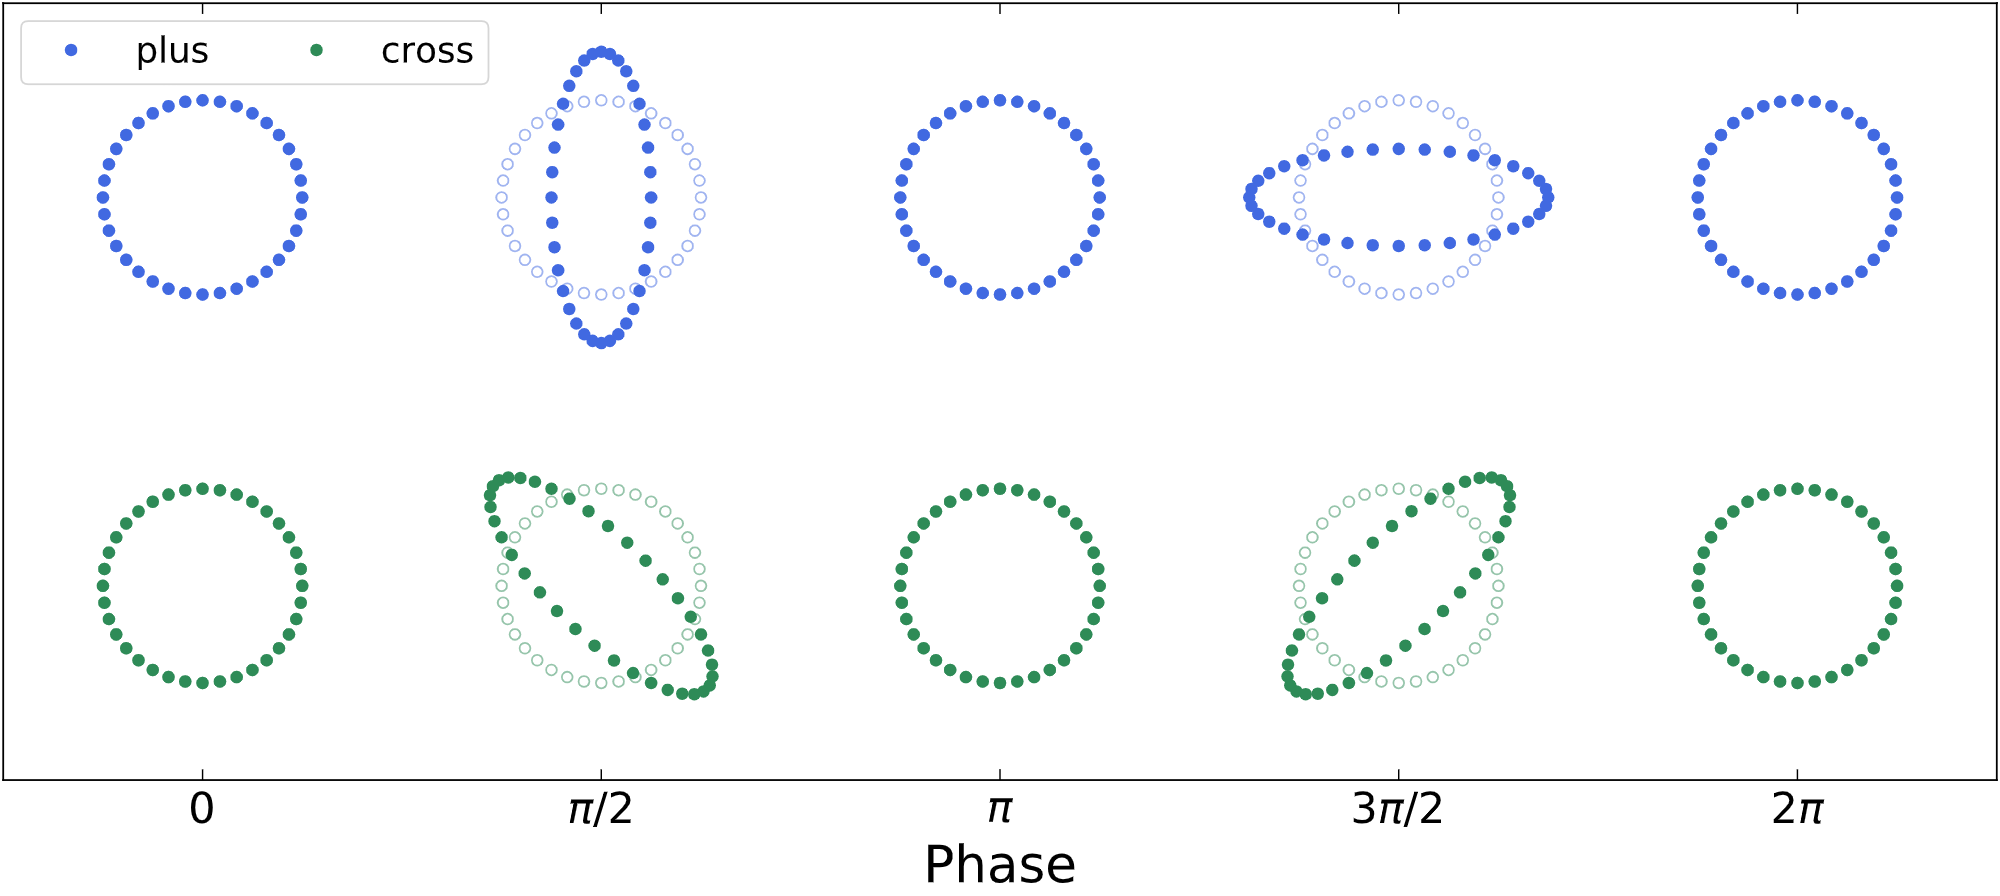
\includegraphics[width=\textwidth]{images/1_general_relativity/polarization.png}
   \caption{The effect of the two polarisations on a ring of test particles~\cite{gw_polarization_plots}.}
   \label{1:fig:ring_of_particles}
\end{figure}
%

\subsection{\label{}Gravitational wave emission in linearised gravity}

We have discussed gravitational waves in our simple linearised gravity with the weak field approximation, in this subsection we will discuss how gravitational waves are generated.

Using the Einstein field equations in the weak-field limit $\Box \Bar{h}^{\mu\nu} = -16 \pi T^{\mu\nu}$ and considering a source at the origin and an observer at the position $\vec{x}^{\prime}$ the solution to the Einstein equations can be obtained using the Green's function,
%
\begin{equation}
    \Bar{h}_{\mu\nu}(t, \vec{x}) = 4 \int d^3 x^{\prime} \frac{T_{\mu\nu}\left(t - ||\vec{x} - \vec{x}^{\prime}||, \vec{x}^{\prime}\right)}{||\vec{x} - \vec{x}^{\prime}||} .
    \label{1:eq:greens_functions}
\end{equation}
%
The gravitational wave emissions can then be approximated using the quadrupole emissions with two assumptions: the observer is far away $\left(||\vec{x} - \vec{x}^{\prime}|| \approx ||\vec{x}|| = r\right)$ and the source velocity is small compared to the speed of light. Equation~\ref{1:eq:greens_functions} then simplifies to
%
\begin{equation}
    \Bar{h}_{\mu\nu}(t, \vec{x}) = \frac{4}{r} \int d^3 x^{\prime} T_{\mu\nu}\left(t - r, \vec{x}^{\prime}\right) .
    \label{1:eq:quadrupole_simplification}
\end{equation}
%
Computing this equation is simpler if we use the TT gauge. Using the laws of conservation of total energy and momentum the right-hand side of equation~\ref{1:eq:quadrupole_simplification} can be expressed as
%
\begin{equation}
    \frac{4}{r} \int d^3 x^{\prime} T_{\mu\nu}\left(t - r, \vec{x}^{\prime}\right) = \frac{2}{r}\frac{\partial^{2}}{\partial t^{2}} \int T_{00} x_{\mu} x_{\nu} d^{3} x^{\prime},
\end{equation}
%
where $T_{00} \approx \rho$, the Newtonian mass density. This redefined expressed is referred to as the \textit{mass quadrupole moment tensor} of the mass distribution,
%
\begin{equation}
    I_{\mu\nu} := \int T_{00} x_{\mu} x_{\nu} d^{3} x^{\prime} ,
    \label{1:eq:quadrupole_moment_tensor}
\end{equation}
%
and when substituted into equation~\ref{1:eq:quadrupole_simplification} get get the \textit{quadrupole formula}
%
\begin{equation}
    h^{TT}_{\mu\nu} = \frac{2}{r} \ddot{I}_{\mu\nu}(t-r).
\end{equation}
The key properties of this equation are the gravitational radiation dependence on the second time derivative of the quadrupole moment tensor, indicating that gravitational waves a produced by rapid changes in the quadrupole moment tensor like accelerations of the masses and they change direction during orbital cycles. Secondly, the gravitational radiation strain falls of inversely to distance $r$ from the source. Finally, encapsulated in the \textit{retarded time} $(t - r)$ is the idea that gravitational waves propagate at the speed of light and the signal received as distance $r$ corresponds to an event that happened $r$ units of time ago.

The total power radiated by a source is the \textit{luminosity flux}  and must be the same as the energy carried by the gravitational waves, due to the conservation of energy. We can obtain the luminosity flux by integrating the energy flux over a sphere with infinite radius from the source We can express the total energy loss rate as:
%
\begin{equation}
    \frac{dE}{dt} = -\mathcal{L},
\end{equation}
%
where $\mathcal{L}$ is the gravitational wave luminosity flux. The luminosity flux at a large distance from the source is given by:
%
\begin{equation}
    L = \frac{1}{5} \left\langle \dddot{Q}^{jk} \dddot{Q}_{jk} \right\rangle,
\end{equation}
%
where $Q_{jk}(t)$ is the mass quadrupole moment of the source, and is defined as:
%
\begin{equation}
    Q_{jk}(t) = \int \rho(t, x^i) \left( x_j x_k - \frac{1}{3} \delta_{jk} x_l x^l \right) d^3x,
\end{equation}
%
where $\rho$ is the mass density distribution and $\delta_{jk}$ is the Kronecker delta. The angular brackets represents averaging over all directions, and $\dddot{Q}_{jk}$ refers to the third time derivative of the quadrupole moment. This shows that any source with a non-vanishing second derivative of its mass quadrupole moment will emit gravitational waves.








\section{\label{1:sec:IFOs}Gravitational wave detection}

% Detection of Gravitational Waves
%     Overview of Detectors: Provide an overview of different types of gravitational wave detectors, focusing on ground-based detectors like LIGO and Virgo, and space-based detectors like LISA.
%     Detector Sensitivity and Noise Sources: Discuss the key factors that influence the sensitivity of detectors, including noise sources like seismic noise, thermal noise, and quantum noise.
%     Interferometry and Signal Extraction: Explain the basic principles of interferometry used in gravitational wave detection and how signals are extracted from the noise.


\subsection{\label{}Laser interferometry}

\subsection{\label{}Increasing detector sensitivity}

\subsection{\label{}Response to gravitational waves}

We have described the effect of gravitational waves on a ring of particles now we will discuss how it is possible to detect these waves on Earth. The induced strain we expect is approximately $\mathcal{O}(10^{-22})$, an almost impossibly small change in length which frames the difficulty of the task of detecting gravitational waves. The detection of gravitational waves is made possible by gravitational wave observatories: the advanced LIGO (aLIGO) detectors in Hanford, USA \& Livingston, USA~\cite{aLIGO:2015}; Virgo in Italy~\cite{aVirgo:2015}; KAGRA in Japan~\cite{KAGRA:2021}; and GEO in Germany~\cite{GEO600:2002}. This section will focus on
the design of the aLIGO interferometers however, the techniques are similar for all detectors. The configuration of aLIGO is described in detail in the 2016 paper~\cite{aLIGO:2015}.

\subsection{\label{1:sec:laser_interferometry}Laser interferometry}

As seen in section~\ref{1:sec:gravitational-propagation}, the physical effects of gravitational waves is a stretching and squeezing of the ring of test particles. We can measure this using laser interferometry allowing the detection of the small
perturbations caused by the presence of \gws in spacetime.

We begin with a basic L-shaped Michelson interferometer, seen in figure \ref{fig:basic_michelson}:

\begin{figure}
   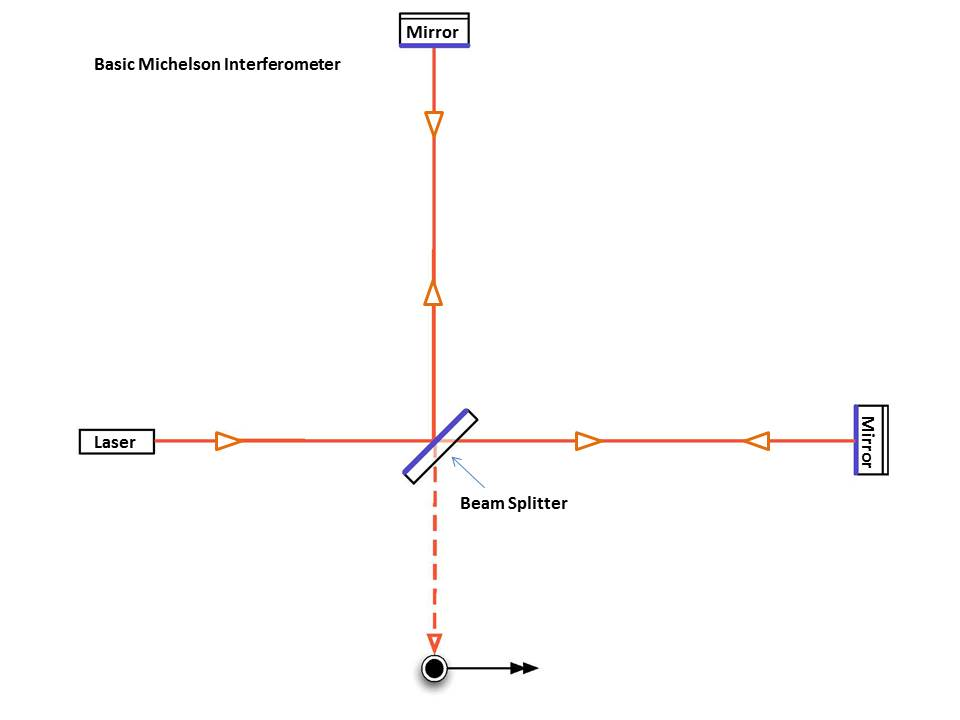
\includegraphics[width=\textwidth]{images/1_general_relativity/Basic_michelson_labeled.jpg}
   \caption{\label{fig:basic_michelson}A basic Michelson interferometer \cite{ligo_ifo}: A laser beam is shone at a beam splitter, the components are sent down equal length perpendicular arms where they reflect off the mirrors at the end, the components are then recombined back at the beam splitter and passed through to the photodetector (black circle) where the interference pattern of the laser is observed.}
\end{figure}

The LIGO detectors are identical in design with arm lengths of 4km, longer arms are able to make more precise measurements, looking at equations \ref{eqn:plus_separation} \& \ref{eqn:cross_separation}, the separation
$\Delta s$ depends on the radius $R$ (analogous to our arm length). We can further increase the distance our laser beam travels by using Fabry-Perot cavities to constantly recycle the laser in the arms. Figure \ref{fig:FP_michelson} shows the inclusion of Fabry-Perot cavities onto our basic Michelson interferometer.

\begin{figure}
   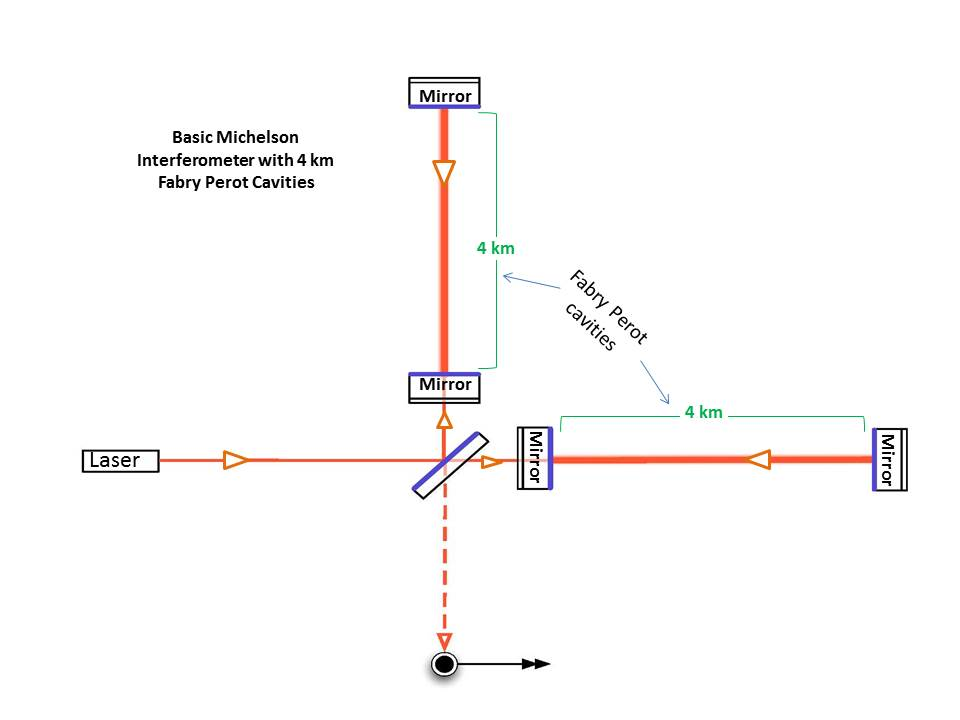
\includegraphics[width=\textwidth]{images/1_general_relativity/Basic_michelson_with_FP_labeled.jpg}
   \caption{\label{fig:FP_michelson}Fabry-Perot cavities \cite{ligo_ifo}: Additional mirrors are placed close to the beam splitter in each arm to allow the laser to traverse the arms many more times, effectively adding distance to our arms.}
\end{figure}

To create Fabry-Perot cavities extra mirrors are placed in each arm close to the beam splitter, these mirrors allow the laser to bounce back and forth within the arm many more times---effectively increasing the distance the laser has travelled. The Fabry-Perot cavities are fully evacuated, further reducing noise from the effects of interactions with particles in the air.

Laser power is continuously built up during this process, the more photons we have in our detector, the greater the resolution at our photodetector. We need to reach a laser power much higher than at the source, the Fabry-Perot
cavities don't provide enough amplification so we need to implement power recycling mirrors prior to the laser reaching the beam splitter. Some of the light from the laser is reflected towards the photodetector from the beam
splitter, the rest of it is sent back to the power recycling mirror. The power recycling mirrors can be seen in figure \ref{fig:IFO}.

\begin{figure}
   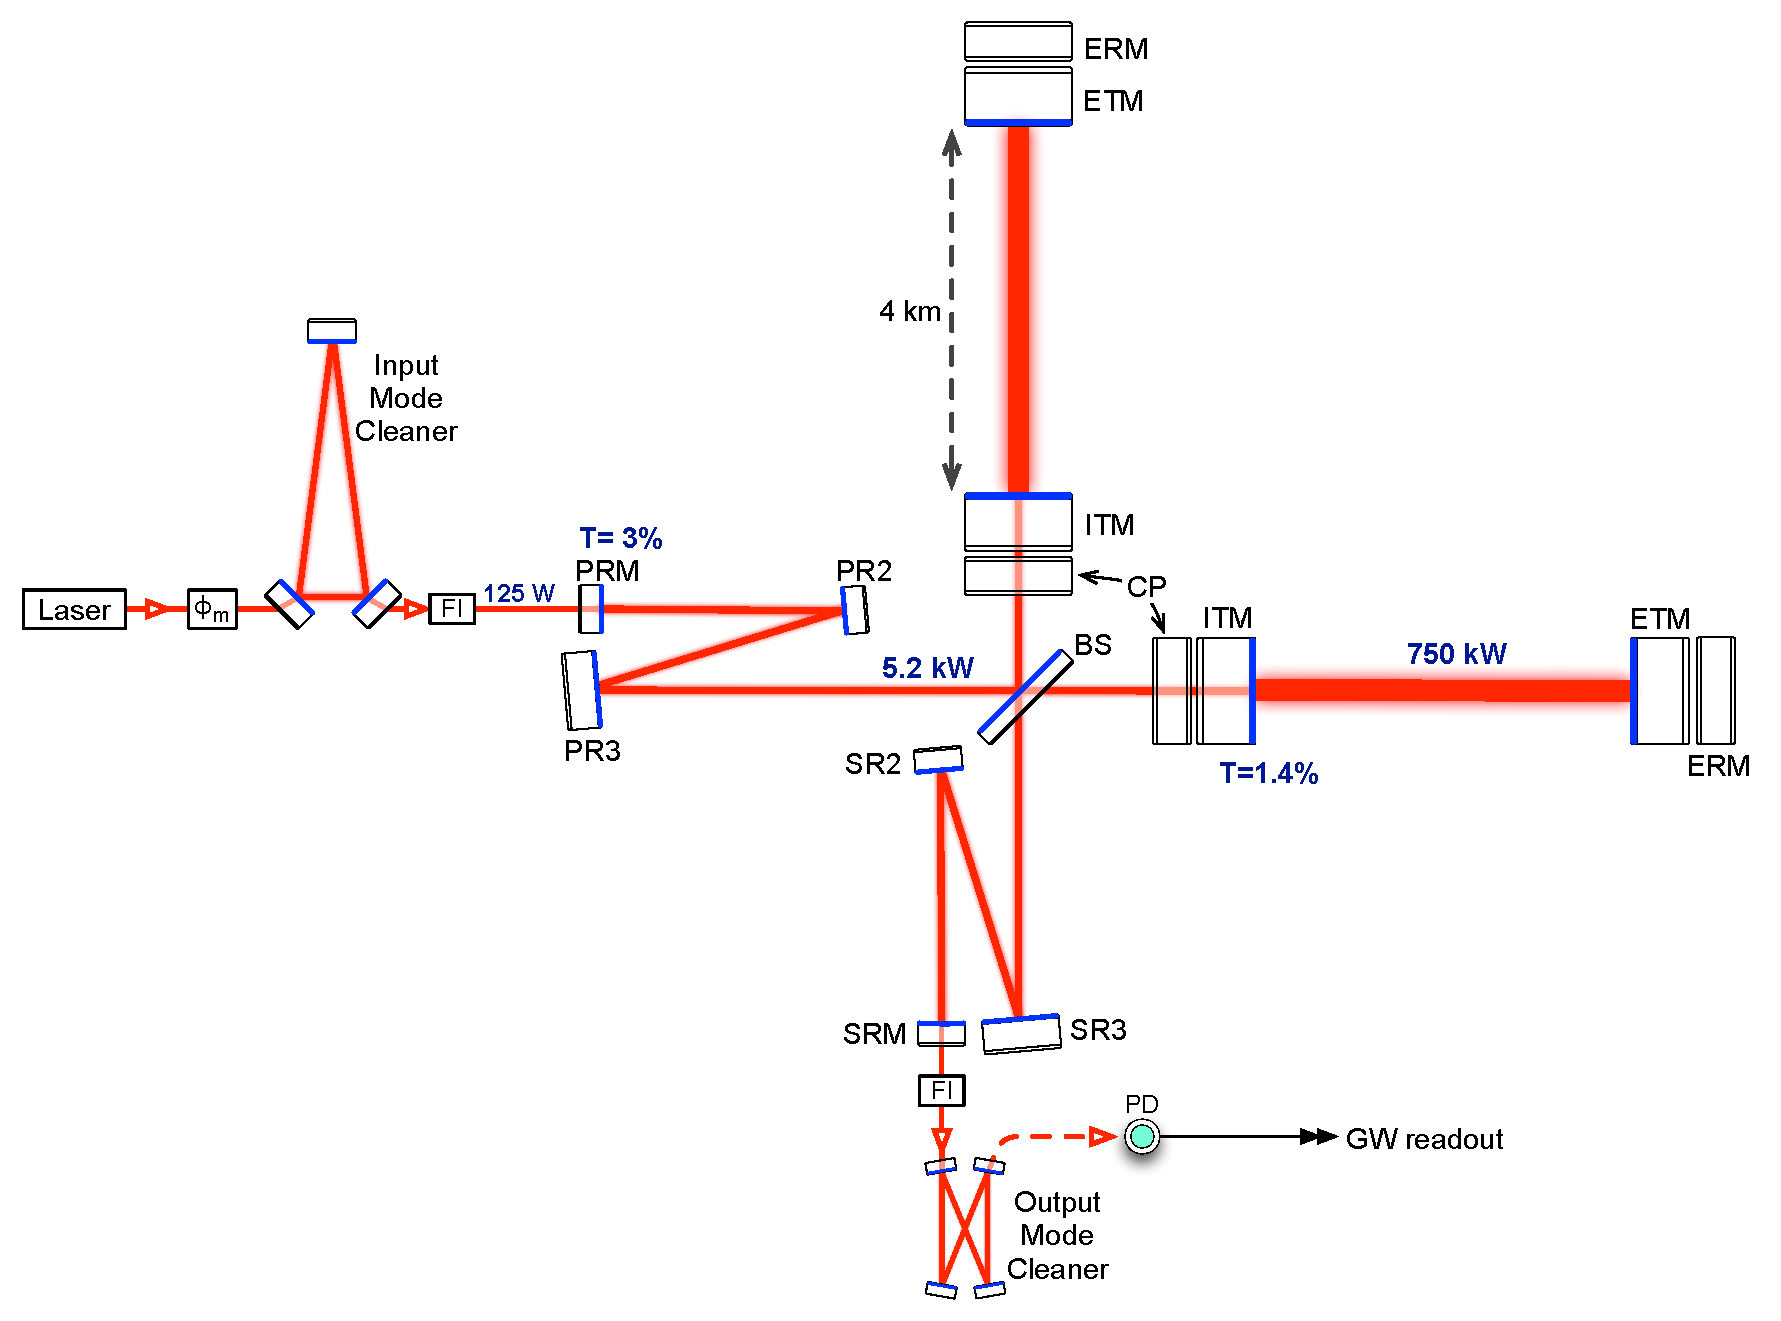
\includegraphics[width=\textwidth]{images/1_general_relativity/IFOdiagram.pdf}
   \caption{\label{fig:IFO}A more complex interferometer diagram \cite{aLIGO:2015}: The Fabry-Perot cavities are formed by the input test mass (ITM) and end test mass (ERM) of each arm, the power recycling mirrors (PRM, PR2, PR3) appear prior to the beam splitter (BS)}
\end{figure}

Within the reference frame of the beam splitter and in the absence of \gws, the distance each laser travels up the arms is equal so that upon returning to the beam splitter, we see a constant interference pattern in the photodetector.
As a \gw propagates through the detector the beam splitter remains at rest but the mirrors at the end of each arm move (in our cartesian coordinate system), the lengths of the arms are now different and the recombination of the two beams will produce a phase difference upon returning back to the beam splitter \cite{thorne_lecture}.










\section{\label{1:sec:CBC}Modelling compact binary coalescences}

















The primary sources of gravitational waves seen by Earth-based gravitational wave detectors are those from compact binary coalescences. Compact binary coalescences (CBC) are the inspiral and merger of two compact objects (black holes or neutron stars), these two objects have typically been locked into a binary star system their whole lives.

We can describe the gravitational waves from a compact binary merger and how these would affect the gravitational wave detectors. We do this with a very simple binary system of two point-like masses using the Newtonian formalism. We commonly refer to the gravitational waves from a source as a `waveform'.

\subsection{\label{1:sec:CBC-parameters}Waveform parameters}

\subsubsection{Intrinsic parameters}
\begin{itemize}
   \item $m_{1}$, the primary component mass
   \item $m_{2}$, the secondary component mass
   \item $\vec{s_{1}}$, the three-dimensional spin vector of the primary component
   \item $\vec{s_{2}}$, the three-dimensional spin vector of the secondary component
\end{itemize}
Here, the subscript $_1$ refers to the more massive object in the binary system, and $_2$ to the less massive one.

\subsubsection{Extrinsic parameters}
\begin{itemize}
   \item $\alpha$, right ascension of the source
   \item $\delta$, declination of the source
   \item $r$, the luminosity distance to the source
   \item $\iota$, the inclination angle between the line of sight and the orbital angular momentum of the binary
   \item $\psi$, the polarization angle of the gravitational wave
   \item $t_{c}$, the time of coalescence
   \item $\phi_{c}$, the coalescence phase
\end{itemize}
The extrinsic parameters affect how the gravitational wave signal is observed.

While these are the fundamental parameters that define a CBC waveform, additional parameters may describe other physical effects. These include tidal deformations, eccentricity, the neutron star equation of state, or potential deviations from general relativity. However, in this work, we will ignore these additional effects and focus on the parameters listed above.

\subsection{\label{}Point mass simplification}

We begin our derivation of the CBC waveform with the simple model of two point objects with masses ($m_{1}$, $m_{2}$) which, when using the Kepler two body p

We use the \textit{quadrupole formula} of a gravitational wave signal
%
\begin{equation}
    h_{\mu\nu}^{TT} = \frac{2}{r} \ddot{I}_{\mu\nu}^{TT} (t-r),
\end{equation}
%
where the superscript $^{TT}$ refers to the transverse traceless gauge, and $\ddot{I}_{\mu\nu}^{TT}$ represents the second order time derivative of the quadrupole moment tensor.

\subsection{\label{}Fourier domain analysis}